% Source for the figure of huffman() (sec. 15.8): the forest of the
% characters a:5, b:9, c:12, d:13, e:16, f:45 before and after the first
% merge (the two least frequent shaded), and the final tree, the left
% edges 0 and the right ones 1, each leaf with its code. Build: make
% figures (in ../build).
\documentclass[border=4pt]{standalone}
\usepackage[T1]{fontenc}
\usepackage{newpxtext,newpxmath}
\usepackage[varqu,varl,scaled=0.95]{zi4}
\usepackage{tikz}
% tikz-ads.tex: the TikZ styles shared by the figures of the memory of the
% manual, \input by each standalone figure: a cell of a vector (cell), the
% cell that an operation touches (touched), a free cell (free), a node of a
% linked structure (node), the labels of indices (index) and of variables
% (var), a pointer (ptr), and \cells and \indices to draw a row of cells.
\usetikzlibrary{arrows.meta,positioning,calc,fit,shapes.multipart}
\definecolor{adsTouched}{RGB}{214,196,236}
\definecolor{adsFree}{RGB}{236,236,236}
\tikzset{
  ads/.style={>={Stealth[length=2mm]},font=\small,
              every node/.append style={inner sep=0pt}},
  cell/.style={draw,minimum width=7mm,minimum height=7mm,
               font=\small\ttfamily,outer sep=0pt},
  touched/.style={cell,fill=adsTouched},
  free/.style={cell,fill=adsFree,text=black!45},
  node/.style={draw,rounded corners=1pt,minimum width=8mm,
               minimum height=6mm,font=\small\ttfamily},
  index/.style={font=\scriptsize\ttfamily,text=black!60},
  var/.style={font=\small\itshape},
  ptr/.style={->,thick}
}
% \cells{name}{x,y}{list}: a row of cells, the first at (x,y), named
% name-0, name-1, ...; each item is text/style, the style one of cell,
% touched and free (e.g., {a/cell,e/touched,/free})
\newcommand{\cells}[3]{%
  \foreach \v/\s [count=\i from 0] in {#3}
    \node[\s] (#1-\i) at ($(#2)+(\i*7mm,0)$) {\v};}
% \indices{name}{n}: the indices 0 .. n-1 under the cells of name
\newcommand{\indices}[2]{%
  \foreach \i in {0,...,\numexpr#2-1\relax}
    \node[index,below=1.2mm of #1-\i] {\i};}

\tikzset{
  lf/.style={rectangle,draw,minimum width=9mm,minimum height=6mm,
             font=\small\ttfamily},
  lt/.style={lf,fill=adsTouched},
  vn/.style={circle,draw,minimum size=7mm,font=\small},
  vt/.style={vn,fill=adsTouched},
  bit/.style={font=\scriptsize\ttfamily,fill=white,inner sep=1pt},
  code/.style={font=\scriptsize\ttfamily,text=black!60}
}
\begin{document}
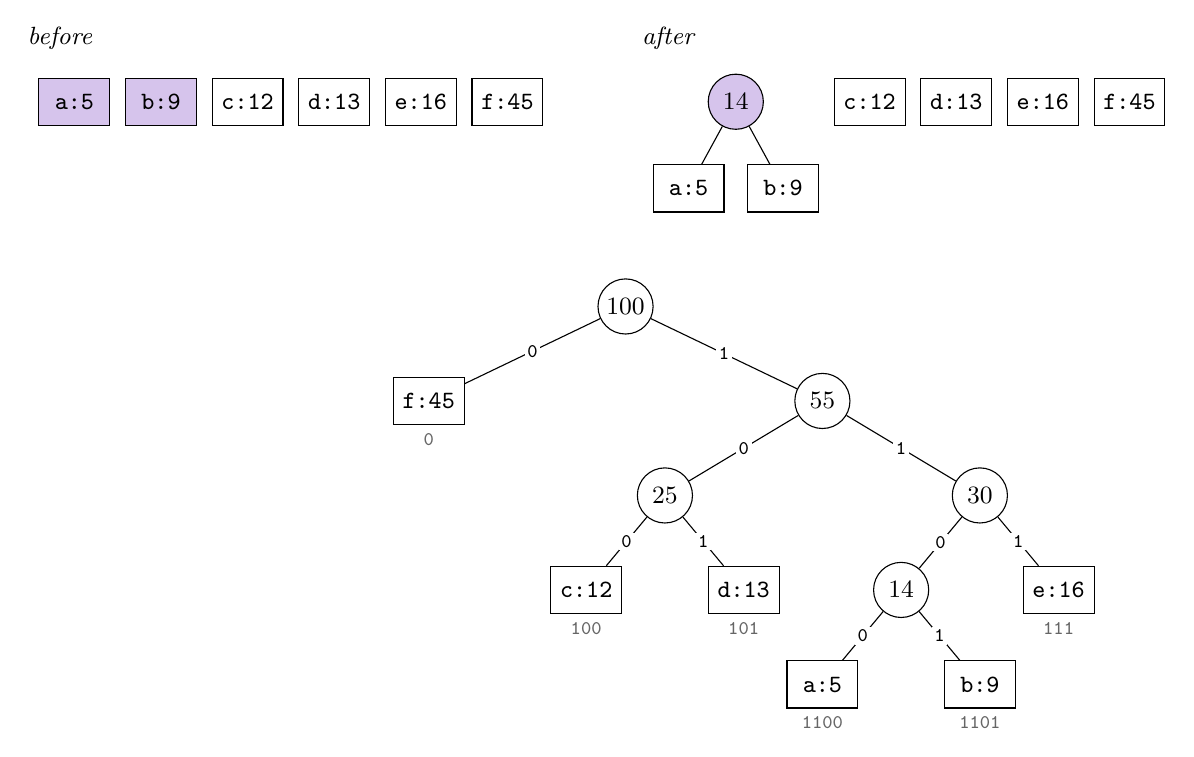
\begin{tikzpicture}[ads]
  % before the first merge
  \node[var,anchor=west] at (-6mm,8mm) {before};
  \foreach \c/\f/\x/\s in {a/5/0/lt,b/9/11/lt,c/12/22/lf,d/13/33/lf,
                           e/16/44/lf,f/45/55/lf}
    \node[\s] at (\x mm,0) {\c:\f};
  % after it
  \node[var,anchor=west] at (72mm,8mm) {after};
  \node[vt] (m) at (84mm,0) {14};
  \node[lf] (ma) at (78mm,-11mm) {a:5};
  \node[lf] (mb) at (90mm,-11mm) {b:9};
  \draw (m) -- (ma); \draw (m) -- (mb);
  \foreach \c/\f/\x in {c/12/101,d/13/112,e/16/123,f/45/134}
    \node[lf] at (\x mm,0) {\c:\f};
  % the final tree
  \begin{scope}[yshift=-26mm,xshift=10mm]
  \node[vn] (r) at (60mm,0) {100};
  \node[lf] (f) at (35mm,-12mm) {f:45};
  \node[vn] (n55) at (85mm,-12mm) {55};
  \node[vn] (n25) at (65mm,-24mm) {25};
  \node[vn] (n30) at (105mm,-24mm) {30};
  \node[lf] (c) at (55mm,-36mm) {c:12};
  \node[lf] (d) at (75mm,-36mm) {d:13};
  \node[vn] (n14) at (95mm,-36mm) {14};
  \node[lf] (e) at (115mm,-36mm) {e:16};
  \node[lf] (a) at (85mm,-48mm) {a:5};
  \node[lf] (b) at (105mm,-48mm) {b:9};
  \draw (r) -- node[bit] {0} (f);
  \draw (r) -- node[bit] {1} (n55);
  \draw (n55) -- node[bit] {0} (n25);
  \draw (n55) -- node[bit] {1} (n30);
  \draw (n25) -- node[bit] {0} (c);
  \draw (n25) -- node[bit] {1} (d);
  \draw (n30) -- node[bit] {0} (n14);
  \draw (n30) -- node[bit] {1} (e);
  \draw (n14) -- node[bit] {0} (a);
  \draw (n14) -- node[bit] {1} (b);
  \foreach \x/\cd in {f/0,c/100,d/101,e/111,a/1100,b/1101}
    \node[code,below=1mm of \x] {\cd};
  \end{scope}
\end{tikzpicture}
\end{document}
